\documentclass[10pt,oneside]{article}

\usepackage[T1]{fontenc}
\usepackage{fontawesome}

\usepackage[paper=a4paper,margin=2cm,bottom=2.5cm]{geometry}
\usepackage[sfdefault,light,condensed]{roboto}
\usepackage[export]{adjustbox}
\usepackage[usenames,dvipsnames,table]{xcolor}

\usepackage{amsmath,amssymb,array,fancyhdr,graphicx,enumitem,lastpage,multicol,tabularx,textcomp,titlesec}
\usepackage{mathtools}

\setlength\extrarowheight{1pt}
\setlength\parindent{0cm}
\renewcommand\headrule{}
\setlength{\footskip}{1.25cm}

\pagestyle{fancy}

\definecolor{BoxHeaderBG}{RGB}{50, 50, 50}
\definecolor{BoxHeaderText}{RGB}{255, 255, 255}

\newcommand{\BoxHeader}[2]{
    \multicolumn{#1}{| >{\bfseries\footnotesize\cellcolor{BoxHeaderBG}\arraybackslash}l |}{
        \textcolor{BoxHeaderText}{#2}
    }
}

\definecolor{ATLHeaderBG}{RGB}{65, 190, 30}
\definecolor{ATLHeaderText}{RGB}{0, 0, 0}

\definecolor{ATLSkillBG}{RGB}{215, 230, 210}
\definecolor{ATLSkillText}{RGB}{0, 0, 0}

\definecolor{DefinitionBoxHeaderBG}{RGB}{30, 30, 110}
\definecolor{DefinitionBoxHeaderText}{RGB}{255, 255, 255}

\definecolor{FormativeHeaderBG}{RGB}{150, 30, 150}
\definecolor{FormativeHeaderText}{RGB}{255, 255, 255}

\definecolor{GlobalContextHeaderBG}{RGB}{255, 255, 150}
\definecolor{GlobalContextHeaderText}{RGB}{0, 0, 0}

\definecolor{KeyConceptHeaderBG}{RGB}{15, 225, 225}
\definecolor{KeyConceptHeaderText}{RGB}{0, 0, 0}

\definecolor{RelatedConceptHeaderBG}{RGB}{15, 170, 170}
\definecolor{RelatedConceptHeaderText}{RGB}{0, 0, 0}

\definecolor{QuestionHeaderBG}{RGB}{240, 240, 240}
\definecolor{QuestionHeaderText}{RGB}{0, 0, 0}

\definecolor{SolutionHeaderBG}{RGB}{225, 150, 110}
\definecolor{SolutionHeaderText}{RGB}{0, 0 , 0}

\definecolor{SummativeHeaderBG}{RGB}{195, 15, 15}
\definecolor{SummativeHeaderText}{RGB}{255, 255, 255}

\newcommand{\ATLHeader}[1]{
    \cellcolor{ATLHeaderBG}\textcolor{ATLHeaderText}{
        \bfseries\footnotesize
        ATL SKILL (#1) \hfill \faGears
    }
}

\newcommand{\ATLSkill}[1]{
    \cellcolor{ATLSkillBG}\textcolor{ATLSkillText}{
        \itshape #1
    }
}

\newcommand{\DefinitionBoxHeader}{
    \cellcolor{DefinitionBoxHeaderBG}\textcolor{DefinitionBoxHeaderText}{
        \bfseries\footnotesize
        DEFINITIONS \hfill \faPencil
    }
}

\newcommand{\FormativeHeader}{
    \cellcolor{FormativeHeaderBG}\textcolor{FormativeHeaderText}{
        \bfseries\footnotesize
        FORMATIVE ASSESSMENT \hfill \faComments
    }
}

\newcommand{\GlobalContextHeader}[1]{
    \cellcolor{GlobalContextHeaderBG}\textcolor{GlobalContextHeaderText}{
        \bfseries\footnotesize
        GLOBAL CONTEXT (#1) \hfill \faGlobe
    }
}

\newcommand{\KeyConceptHeader}[1]{
    \cellcolor{KeyConceptHeaderBG}\textcolor{KeyConceptHeaderText}{
        \bfseries\footnotesize
        KEY CONCEPT (#1) \hfill \faKey
    }
}

\newcommand{\RelatedConceptHeader}[1]{
    \cellcolor{RelatedConceptHeaderBG}\textcolor{RelatedConceptHeaderText}{
        \bfseries\footnotesize
        RELATED CONCEPT (#1) \hfill \faLink
    }
}

\newcommand{\SolutionHeader}[1]{
    \cellcolor{SolutionHeaderBG}\textcolor{SolutionHeaderText}{
        \bfseries\footnotesize 
        #1 \hfill \faPaste
    }
}

\newcommand{\SummativeHeader}{
    \cellcolor{SummativeHeaderBG}\textcolor{SummativeHeaderText}{
        \bfseries\footnotesize
        SUMMATIVE ASSESSMENT \hfill \faCheck
    }
}

\newcounter{QuestionCounter}

\newcommand{\QuestionBox}[1]{
    \stepcounter{QuestionCounter}
    \cellcolor{QuestionHeaderBG}\textcolor{QuestionHeaderText}{
        {\bfseries\scriptsize Q\theQuestionCounter} #1
    }
}

\newcommand{\boxwidth}{\linewidth}

\lhead{\scriptsize\texttt{U\UnitNumber: \UnitTitle \\ L\LessonNumber: \LessonTitle}}
\rhead{\scriptsize\ttfamily [DESIGN/\CourseName/U\UnitNumber/L\LessonNumber]\\\ }

\lfoot{
\includegraphics[height=2cm,valign=c]{Files/logo}}
\cfoot{\footnotesize DESIGN/\CourseName/U\UnitNumber/L\LessonNumber\ | \LessonTitle \\ Woodstock School | Mussoorie, Uttarakhand, India}
\rfoot{
\includegraphics[height=2cm,valign=c]{Files/ib-world-school-logo-1-colour}}

\titleformat{\section}{\normalfont\Large\bfseries}{}{0em}{}[{\titlerule[0.5pt]}]
\titleformat{\subsection}{\normalfont\large\bfseries}{}{0em}{}


\usepackage{tikzsymbols}
\usepackage[arrowmos]{circuitikz}

\usetikzlibrary{calc}

\def\CourseName{MYP3}

\def\LessonNumber{05}
\def\LessonTitle{The Transistor}

\def\UnitNumber{01}
\def\UnitTitle{Circuits \& Electronics}

\begin{document}
    \textbf{\large Name: } \rule{12cm}{0.5pt} \hfill \textbf{\large Section: } \rule{1cm}{0.5pt}

    \begin{center}
        \huge\bfseries
        \LessonTitle
    \end{center}

    \section{Before You Begin}
    This lesson represents the final lesson in this unit where you will learn about new electronic components. The \emph{transistor} is a very important component used in nearly all modern electronics. 
    
    \medskip
    Answer each of the following questions relating our Global Context and Related Concept to this important component.

    \bigskip
    \begin{tabularx}{\boxwidth}{| X |}
        \hline
        \GlobalContextHeader{Orientation in Space \& Time}\\\hline
        \cellcolor{QuestionHeaderBG}\textcolor{QuestionHeaderText}{
            The fundamental electronic component we will be learning about this lesson, the \emph{transistor}, is the primary component responsible for a computer's ability to perform the calculations and data manipulations required by every task we give it. \emph{Moore's Law}, an important concept in computing, states that the number of transistors in an integrated circuit, such as a computer's main processor, roughly doubles every two years.
        } \\[1.5cm]
        \cellcolor{QuestionHeaderBG}\textcolor{QuestionHeaderText}{Although this idea was initially proposed by Gordon Moore in 1965 and predited to last a decade, it had held mostly true every since, accurately predicting the exponential growth in speed and power of computer systems over the past 55 years. Nonetheless, many experts expect this trend to end in the next decade.}\\[1cm]
        \QuestionBox{How would you anticipate the potential slow in growth of speed and power of computer systems to impact the tech industry?}\\\hline
        \ \\[6cm]\hline
    \end{tabularx}
    
    \medskip
    \begin{tabularx}{\boxwidth}{| X |}
        \hline
        \RelatedConceptHeader{Invention}\\\hline
        \QuestionBox{Do you think this slow in growth will lead to new inventions that supersede computers within the next few decades? Why or why not?}\\\hline
        \ \\[6cm]\hline
    \end{tabularx}

    \pagebreak

    \section{Technical Background}
    The transistor is a fairly complex device. As such, this lesson represents only a small fraction of the knowledge you would need to use them effectively in original circuits. Nonetheless, you'll be able to explore a basic use of the transistor necessary for future projects in the following sections and example circuits.

    \medskip
    The development of the transistor represented a very important turning point even within the electronics industry. Various documentaries and other historical accounts are linked for you on the course stream, if you wish to know more.
    % Transistor Definition
    \subsection{Transistor Types}
    % Types of Transistors
    % - Bipolar Junction: Current Amplification    
    % -- PNP v. NPN
    % - Field Effect Transistor: Voltage Amplification
    % -- Mosfet
    \begin{tabularx}{\boxwidth}{| >{\bfseries}p{0.15\boxwidth} | X | >{\centering\arraybackslash}p{0.15\boxwidth} | >{\centering\arraybackslash}p{0.15\boxwidth}| }
        \hline
        \BoxHeader{1}{Name} & \BoxHeader{1}{Description} & \BoxHeader{1}{Symbol} & \BoxHeader{1}{Example} \\\hline
        Bipolar Junction (BJT) & A \emph{bipolar junction transistor} is what is traditionally referred to when a ``transistor'' is mentioned. It is considered a \emph{current amplifier} as small fluctuations in its \emph{base pin} can allow large current to flow from its \emph{collector} to its \emph{emitter}.
        
        \medskip
        The symbol and example on the right are for a \emph{NPN Bipolar Junction Transistor}, the type of transistor that will be in your electronics kit.
        & \raisebox{-2.25cm}{\tikz \draw (0, 0) node[npn] {} (-0.25, 0) circle (0.6);} & \raisebox{-2.25cm}{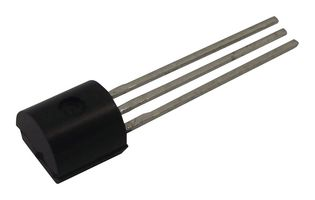
\includegraphics[width=2.5cm]{Extras/npnbjt}} \\\hline
        Field Effect (FET) & A \emph{field effect transistor} is one of the most important and widely used type of transistors in modern electronic devices, such as cell phones and computers. They are considered \emph{voltage amplifiers}, as small voltages applied to their \emph{gate pins} allow large voltages to flow between their \emph{drain pins} and \emph{source pins}.

        \medskip
        The symbol and example on the right are for a typical \emph{Metal-Oxide Field Effect Transistor (MOSFET)}.
        & \raisebox{-2.25cm}{\tikz \draw (0, 0) node[nmos] {} (-0.25, 0) circle (0.6);} & \raisebox{-2.5cm}{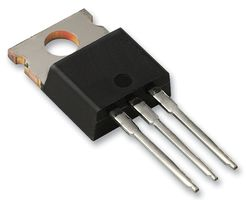
\includegraphics[width=2.5cm]{Extras/mosfet}} \\\hline
    \end{tabularx}

    \subsection{Transistors as Switches}
    One simple use for a transistor is as an electronic \emph{switch}. Unlike the pushbutton switches explored earlier, transistors can control the flow of electricity almost autonomously through the application of a small amount of current to its \emph{base pin}.

    \subsubsection*{The Pins of a NPN BJT}

    \begin{minipage}{0.6\boxwidth}
        A transistor is a \emph{tripole} component, meaning it has three pins to connect within a circuit. The diagram on the right labels the three pins as the \emph{collector}, \emph{base}, and \emph{emitter}.

        \medskip
        In a circuit, the flow of electricity should be considered as passing through the collector to the emitter. A small, positive current to the base pin will allow for this flow of electricity.
    \end{minipage}
    \begin{minipage}{0.1\boxwidth}
    \ 
    \end{minipage}
    \begin{minipage}{0.25\boxwidth}
        \begin{circuitikz}
            \draw (0, 0) node[npn,scale=1.25] (npn) {}
                (npn.base) node[anchor=east] {Base ($+$)}
                (npn.collector) node[anchor=south] {Collector ($+$)}
                (npn.emitter) node[anchor=north] {Emitter ($-$)};
            \draw (-0.25, 0) circle (0.75);
        \end{circuitikz}
    \end{minipage}

    \subsubsection*{Leaking Current}
    It is important to note that unlike with physical switches where the flow of electricity when they are \emph{open} is nearly impossible, a bipolar junction transistor often ``leaks'' a small amount of current across its collector/emitter pins, even when no current is being applied to its base pins. This will likely be evident in the example circuit given in the next section.

    \bigskip
    \begin{tabularx}{\boxwidth}{| X |}
        \hline
        \ATLHeader{Communication Skills}\\\hline
        \ATLSkill{...make inferences and draw conclusions...}\\\hline
        \QuestionBox{Why might the small amount of current leakage that can occur in a bipolar junction transistor make them problematic for sensitive equipment and applications?}\\\hline
        \ \\[1.25cm]\hline
    \end{tabularx}
    \pagebreak

    \section{Developing Technical Skills}

    \subsection{Circuit \#14}
    This circuit uses a transistor triggered by a very small electrical current as a ``switch'' to turn on the LED. Once built, you will be able to turn on the LED by bridging the gap between the two open ends with your finger.

    \bigskip
    \begin{center}
        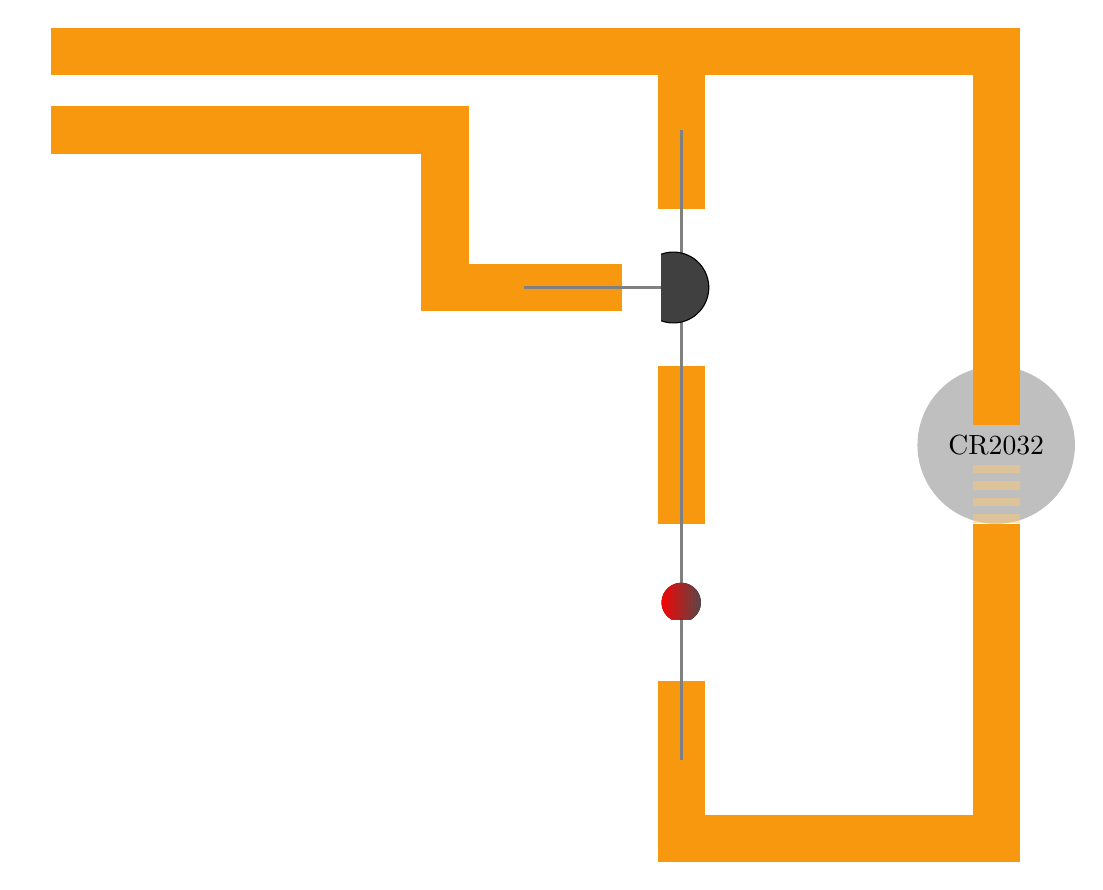
\begin{tikzpicture}
            \draw[line width=6mm,YellowOrange]  
                (12, 1) |- (0, 5)
                (0, 4) -| (5, 2) -- (7.25, 2)
                (8, 5) -- (8, 3)
                (8, 1) -- (8, -1)
                (8, -3) -- (8, -5) -| (12, -1)            
            ;

            \fill[black!25] (12, 0) circle (10mm);            
            \draw[line width=6mm, dashed,YellowOrange!50,draw opacity=0.5] (12, -0.25) -- (12, -1);
            \draw[line width=6mm,YellowOrange] (12, 0.25) -- (12, 1);
            \node[align=center] at (12, 0) {CR2032};

            \begin{scope}[xshift=8cm,yshift=2cm]
                \draw[black!50,very thick] (0, 2) -- (0, -2);
                \draw[black!50,very thick] (0, 0) -- (-2, 0);
                \draw[fill=black!75] (-0.1, 0) +(110:0.45cm) arc (110:-110:0.45cm);    
            \end{scope}

            \draw[very thick,black!50] (8, 0) -- (8, -4);
            \fill[left color=red, right color=black!70] ([shift=(-60:2.5mm)]8,-2) arc (-60:240:2.5mm);
        \end{tikzpicture}
    \end{center}

    \bigskip
    \begin{tabularx}{\boxwidth}{| X |}
        \hline
        \ATLHeader{Communication Skills}\\\hline
        \ATLSkill{...make inferences and draw conclusions...}\\\hline
        \QuestionBox{Why does triggering the above circuit using your finger represent a small amount of current, even though you are still using energy from the 3V battery?}\\\hline
        \ \\[2.75cm]\hline
        \ATLHeader{Creative Thinking Skills}\\\hline
        \ATLSkill{...develop improvements to existing machines, media, and technologies...}\\\hline
        \QuestionBox{Although we are using your finger to trigger the above circuit, anything that would cause a small current to flow into the base pin of the transistor would work to switch the LED on. Describe a few other uses for the above (or similiar) circuits.}\\\hline
        \ \\[2.75cm]\hline
    \end{tabularx}

    \pagebreak
    
    \begin{tabularx}{\boxwidth}{| X |}
        \hline
        \FormativeHeader\\\hline
        \QuestionBox{Hold hands with a partner and have each of you touch a single side of the ``switch'' from Circuit \#14 above. Does the behaviour of the circuit meet your expectations? Explain why or why not.}\\\hline
        \ \\[5cm]\hline
        \QuestionBox{Use a multimeter to determine how much resistance and current your body and you and your partner together produce.}\\\hline
        \ \\[2cm]\hline
        \ATLHeader{Communication Skills}\\\hline
        \ATLSkill{...make inferences and draw conclusion...}\\\hline
        \QuestionBox{Determine the maximum number of people you can link by holding hands that will still operate the transistor in the above circuit. What properties of each individual do you think impacts this number?}\\\hline
        \ \\[5cm]\hline
        \ATLSkill{...use and interpret a range of discipline specific terms and symbols...}\\\hline
        \QuestionBox{Draw the circuit diagram for Circuit \#14 above.}\\\hline
        \ \\[5cm]\hline
    \end{tabularx}

    \pagebreak
    \section{Reflections}
    \begin{tabularx}{\boxwidth}{| X |}
        \hline
        \ATLHeader{Communication Skills}\\\hline
        \ATLSkill{...make inferences and draw conclusions...}\\\hline
        \QuestionBox{Why is it important that a transistor can be operated using extremely low currents?}\\\hline
        \ \\[4cm]\hline
        \QuestionBox{Transistors are extremely important for modern computing, being used for calculations, logic processing, and memory storage. What aspects of a transistor's function allows it to hold such a key role in modern technology?}\\\hline
         \ \\[4cm]\hline
    \end{tabularx}

    \bigskip
    \begin{tabularx}{\boxwidth}{| X |}
        \hline
        \QuestionBox{What aspect of this lesson was the most challenging for you? How did you overcome that challenge?}\\\hline
        \ \\[3.5cm]\hline
        \QuestionBox{Select the option which best reflects how confident you are in applying what you have learend in this lesson.}\\\hline
        \, \hfill \Sadey[5][orange] \hfill \Neutrey[5][gray] \hfill \Smiley[5][cyan] \hfill \,\\\hline
        \QuestionBox{What additional questions do you still have about this lesson's content?}\\\hline
        \ \\[3.5cm]\hline
    \end{tabularx}   
\end{document}